\documentclass[main.tex]{subfiles}
\begin{document}
\chapter{Introduction}
\label{ch:intro}
\section{Our Team}
Waterloop is a team of ambitious students from the University of Waterloo who have been working to design and build prototype Hyperloop pods since September 2015 with the goal to compete in SpaceX's Hyperloop Pod Competitions. We hope to represent Canada's leading innovation on the world stage at Competition III.

The team is based in Waterloo, Ontario, Canada’s largest technology innovation hub. Waterloop has members studying in fields ranging from engineering to arts to environment to business, and our members also represent over 20 countries of origin. Our diverse team is united under the common goal of building a pod that is able to not only do well in competition, but can eventually be implemented in Canada's transportation infrastructure. We believe Hyperloop has the potential to link together the economy and shrink the world in a faster, cleaner, and more efficient way.

We are excited to build this cutting-edge technology with the potential to revolutionize - or even trivialize - the concept of distance. On a personal level, it has been an extraordinary experience teaching and learning technical and administrative skills, creating strong organizational and engineering practices, and, most of all, engaging in amazing teamwork. We are also proud to be actively promoting programs that will bring our own life-changing experiences to a wider community, including work with HeForShe Waterloo and hosting educational events to promote the importance of STEM in Canada's future. We hope to be a leader in Canada's surge back into the forefront of innovation.

\subsection{Administrative Facts}
\begin{itemize}
\item Performed a complete rebranding, resulting in the logo which can be seen at the bottom of each page.
\item Confirmed over \$30,000 in sponsorship, with much more under discussion.
\item Reached nearly 4000 likes on Facebook, and less than a week after opening recruitment have received almost 50 applications.
\item Gained support at many levels of the University administration through periodic pod showcases and tours.
\end{itemize}

\subsection{Team Members Fall 2017}
Due to the University of Waterloo co-op system, our team rotates approximately every four months.

\begin{flushleft}
\begin{tabularx}{\linewidth}{@{}XXX@{}}
	\begin{center}\large{Directors}\end{center}
    \begin{itemize}[label={},noitemsep]
        \item \textbf{Clive Chan}, Technical
        \item \textbf{Jason Pan}, Administrative
    \end{itemize}
    &
    \begin{center}\large{Advisors}\end{center}
    \begin{itemize}[label={},noitemsep]
        \item \textbf{Serhiy Yarusevych}, Faculty
        \item \textbf{Victor Qian}, Alumnus
    \end{itemize}
    &
    \begin{center}\large{Integration Leads}\end{center}
    \begin{itemize}[label={},noitemsep]
        \item Ben Tonita
        \item Jimmy Zhou
    \end{itemize}
\end{tabularx}
\newpage
\begin{center}\large{Technical Team Leads}\end{center}
\begin{tabularx}{\linewidth}{@{}XXX@{}}
    \begin{center}\large{Mechanical}\end{center}
    \begin{itemize}[label={},noitemsep]
    \item \textbf{Jimmy Zhou}
    \item \textbf{Ben Tonita}
    \item \textbf{Donovan Kwong, Friction~Drive}
    \item \textbf{Dallyn Wynnychuk, Friction~Drive}
    \end{itemize}
    &
    \begin{center}\large{Software}\end{center}
    \begin{itemize}[label={},noitemsep]
    \item \textbf{Deep Dhillon}
    \item \textbf{Ruslan Nikolaev}
    \end{itemize}
    &
    \begin{center}\large{Electrical}\end{center}
    \begin{itemize}[label={},noitemsep]
    \item \textbf{Chawthri Kanagarasa}
    \end{itemize}
\end{tabularx}
\begin{center}\large{Administrative Team Leads}\end{center}
\begin{tabularx}{\linewidth}{@{}XXX@{}}
    \begin{center}\large{Sponsorship}\end{center}
    \begin{itemize}[label={},noitemsep]
    \item \textbf{Nicholas Jelich}
    \end{itemize}
    &
    \begin{center}\large{Media}\end{center}
    \begin{itemize}[label={},noitemsep]
    \item \textbf{Natalia Zigante}
    \end{itemize}
    &
    \begin{center}\large{Finance}\end{center}
    \begin{itemize}[label={},noitemsep]
    \item \textbf{Nafee Hasan}
    \end{itemize}
\end{tabularx}
\end{flushleft}

\begin{center}\LARGE{Team Roster}\end{center}
\begin{multicols}{3}
 \begin{itemize}[label={},noitemsep]
     \item \small{Aayush Sharma}
     \item {Abdelrahman Ayad}
     \item {Aditya Arora}
     \item {Adrian Fagarasanu}
     \item {Ahmed Al-Hasani}
	 \item {Ambareesh Balaji}
     \item {Amy Sun}
	 \item {Anthony Fabian}
     \item {Archer Zhang}
	 \item {Armanit Garg}
     \item {Arnav Garcha}
	 \item {Attilio Ravani}
     \item {Ayush Kapur}
	 \item {Ben Tonita}
     \item {Benjamin Li}
	 \item {Bob Wei}
     \item {Callum McCracken}
	 \item {Casey Garcia}
     \item {Chawthri Kanagarasa}
	 \item {Chun Hang Lau}
     \item {Clive Chan}
	 \item {Colin Batchellor}
     \item {Connor Nicholls}
	 \item {Cyril Vaidhyan}
     \item {Dallyn Wynnychuk}
	 \item {Daniel Ingriselli}
     \item {Daniyal Shaikh}
	 \item {Deep Dhillon}
     \item {Donovan Kwong}
	 \item {Edmond Lu}
     \item {Edwin Zhang}
	 \item {Egemen Guray}
     \item {Emile Patry}
	 \item {Emrys Halbertsma}
     \item {Eniife Elebute}
	 \item {Gianni Recupero}
     \item {Greg Hill}
	 \item {Griffin Barniutt}
     \item {Griffin Keglevich}
	 \item {Heather D'Souza}
     \item {Ibrahim Irfan}
     \item {Illya Myshakov}
	 \item {Imad Azzam}
     \item {Isabel Zhu}
	 \item {James Lu}
     \item {James Ro}
	 \item {Jason Pan}
     \item {Jeff Niu}
	 \item {Jenarth Jegatheeswaran}
     \item {Jimmy Zhou}
	 \item {Jonathan Lee}
     \item {Jordan Lin}
	 \item {Justin Gorvett}
     \item {Justin Hammond}
	 \item {Justin Pu}
     \item {Justin Schaper}
	 \item {Kaeun Kim}
     \item {Kelvin Tezinde}
	 \item {Kunal Jhaveri}
	 \item {Laura Chambers}
     \item {Lily Hwang}
	 \item {Loic Murumba}
     \item {Mathieu Godin}
	 \item {Melissa Tran}
     \item {Monica Chung}
	 \item {Nafee Hasan}
     \item {Namitra Kalicharran}
	 \item {Natalia Zigante}
     \item {Natasha Poley}
	 \item {Navraj Singh Chhina}
     \item {Navreet Dhillon}
	 \item {Neil McClean}
     \item {Nicholas Jelich}
	 \item {Nicole Rosario}
     \item {Noah Ford}
	 \item {Pascal Voyer-Nguyen}
     \item {Promit Barua}
	 \item {Ruslan Nikolaev}
     \item {Saif Hafeez}
	 \item {Sam MacLeod}
     \item {Shubham Patil}
	 \item {Shun Rao}
     \item {Stefan Sing}
	 \item {Stephanie Mills}
     \item {Steven Kozachuk}
     \item {Turja Aninda}
	 \item {Tushar Sekhri}
     \item {Tyler Zhang}
	 \item {Urooj Khaleeli}
     \item {Victor Qian}
	 \item {William James Ngana}
     \item {William Xian}
	 \item {William Yan}
     \item {Yazan Obeidi}
	 \item {Yi Dong}
     \item {Yingning Gui}
	 \item {Zhaoxin Zhang}
     \item {Ziyang Huang}
\end{itemize}
\end{multicols}
\newpage
\subsection{Sponsors}
Thanks to all our sponsors, past and present.
\begin{multicols}{3}
    \begin{itemize}[label={},noitemsep]
    \item {Babylon VR}
    \item {BALLUFF}
    \item {Boko}
    \item {Camino Modular Systems}
    \item {Caro Systems}
    \item {Communitech}
    \item {Dassault Systems}
    \item {Eagle CAD}
    \item {GroveWare}
    \item {Heins Management Consulting Inc.}
    \item {IBI}
    \item {iDream Labs}
    \item {Infinity Testing}
    \item {Inksmith}
    \item {Javelin}
    \item {Kik}
    \item {League}
    \item {Leggett and Platt}
    \item {LOT}
    \item {Maplesoft}
    \item {Masrio Architects}
    \item {Miltera}
    \item {MMOSER Associates}
    \item {Naylor}
    \item {Paypal}
    \item {Phidon}
    \item {Routes Transport Group}
    \item {Sandford Fleming Foundation}
    \item {Silver Star}
    \item {Waterloo Architecture Graduates}
    \item {Sourced}
    \item {Sustainable TO}
    \item {University of Waterloo}
    \item {UW Faculty of Engineering}
    \item {UW Faculty of Science}
    \item {UW EngSoc}
    \item {WEEF}
    \item {William J. Pristanski}
    \end{itemize}
\end{multicols}

\subsection{Acknowledgements}

We are grateful to many people and organizations that have helped make this possible:
\begin{itemize}
	\item The University for its constant support of our mission, especially Sandra Banks and the Sedra Student Design Centre, who host our primary work location;

	\item All of our incredible sponsors from all industries, without whose monetary and in-kind support we'd have merely a fun idea with nothing to show for it;

	\item Student and faculty individuals and organizations from around the University for support in so many ways, including Waterloo Formula Electric, Techyon, EngSoc, MathSoc, and many more;

	\item and finally SpaceX, Elon Musk, and the Hyperloop Competition volunteers for organizing an event that will go down in history as starting a transportation revolution.

	\item Additionally, we acknowledge that we live and work on the traditional territory of the Attawandaron (Neutral), Anishinaabeg and Haudenosaunee peoples. The University of Waterloo is situated on the Haldimand Tract, the land promised to the Six Nations that includes ten kilometers on each side of the Grand River.
\end{itemize}

\newpage
\section{History}
\begin{itemize}

\item Summer 2015:
\begin{itemize}
    \item Formation of the team.
    \item Officially registered as a University of Waterloo Student Engineering Team.
\end{itemize}

\item Fall 2015:
\begin{itemize}
    \item Preliminary design briefing and evaluation by SpaceX. One of the 1200 teams entering the competition.
\end{itemize}

\item Winter 2016:
\begin{itemize}
    \item Final design briefing and evaluation by SpaceX.
    \item Hyperloop Design Weekend at Texas A\&M. One of the 31 teams around the world to advance.
\end{itemize}

\item May 2016:
\begin{itemize}
    \item Subsystem R\&D and feasibility analysis.
    \item Granted a private workshop at the Sedra Smith Design Centre at the University of Waterloo.
\end{itemize}

\item June 2016:
\begin{itemize}
    \item Designing and building rigs for subsystem testing - air levitation, eddy current braking, operating electronics in a vacuum.
\end{itemize}

\item August 2016:
\begin{itemize}
    \item Parts sourcing.
    \item Frame fabrication.
    \item Construction of a low speed test track.
    \item Finalizing Goose I subsystem design.
\end{itemize}

\item October 2016:
\begin{itemize}
    \item Achieved air levitation.
    \item Development of embedded and communication systems.
    \item Vacuum chamber testing.
    \item Launching a Kickstarter campaign to supplement sponsorship.
\end{itemize}

\item November 2016:
\begin{itemize}
    \item Successfully raised CA\$43,416 with 507 backers on Goose I Kickstarter campaign.
\end{itemize}

\item December 2016:
\begin{itemize}
    \item High speed performance testing.
    \item System optimization.
    \item Reliability and safety testing.
\end{itemize}

\item January 2017:
\begin{itemize}
    \item Attending SpaceX competition with Goose I pod.
\end{itemize}

\item February 2017:
\begin{itemize}
    \item Analyzing feedback from the SpaceX competition.
\end{itemize}

\item March 2017:
\begin{itemize}
    \item Beginning the build of Goose II pod. Working on overall system improvements and overhaul of multiple subsystems based on feedback from competition.
\end{itemize}

\item May 2017:
\begin{itemize}
    \item Developing a brand new embedded and communication systems.
    \item Completing the assembly of Magnetic Wheels for Goose II.
    \item Starting Goose II shell design process.
    \item Starting the final assembly of the pod.
\end{itemize}

\item June 2017:
\begin{itemize}
    \item Vibrational testing of the Goose II to find and eliminate any resonance frequencies.
    \item Testing new embedded systems elements in vacuum.
    \item Integrating required sensors into embedded systems.
    \item Testing communication systems and data visualization on front-end.
    \item Completing static and dynamic levitation tests.
\end{itemize}

\item July 2017:
\begin{itemize}
    \item Goose II unveil.
    \item Beginning preparations for SpaceX Competition 2.
    \item Implementing redundancy checks and safety enhancing features in software.
    \item Second vibrational testing to tune shock absorption for competition.
\end{itemize}

\item August 2017:
\begin{itemize}
    \item Tuning speed controllers for Magnetic Wheels.
    \item Finalizing internal wiring of the pod.
    \item Completing required administrative arrangements for the competition and transportation of the pod to SpaceX headquarters in California.
    \item Shipping the pod to California.
    \item Attending SpaceX Competition 2.
\end{itemize}

\end{itemize}

\incgraph[documentpaper]
  	[width=\paperwidth,height=\paperheight]{images/front_off_top-level.png}

\chapter{Top-Level Design}
\label{ch:top-level-design}
    \begin{figure}[H]
        \centering
        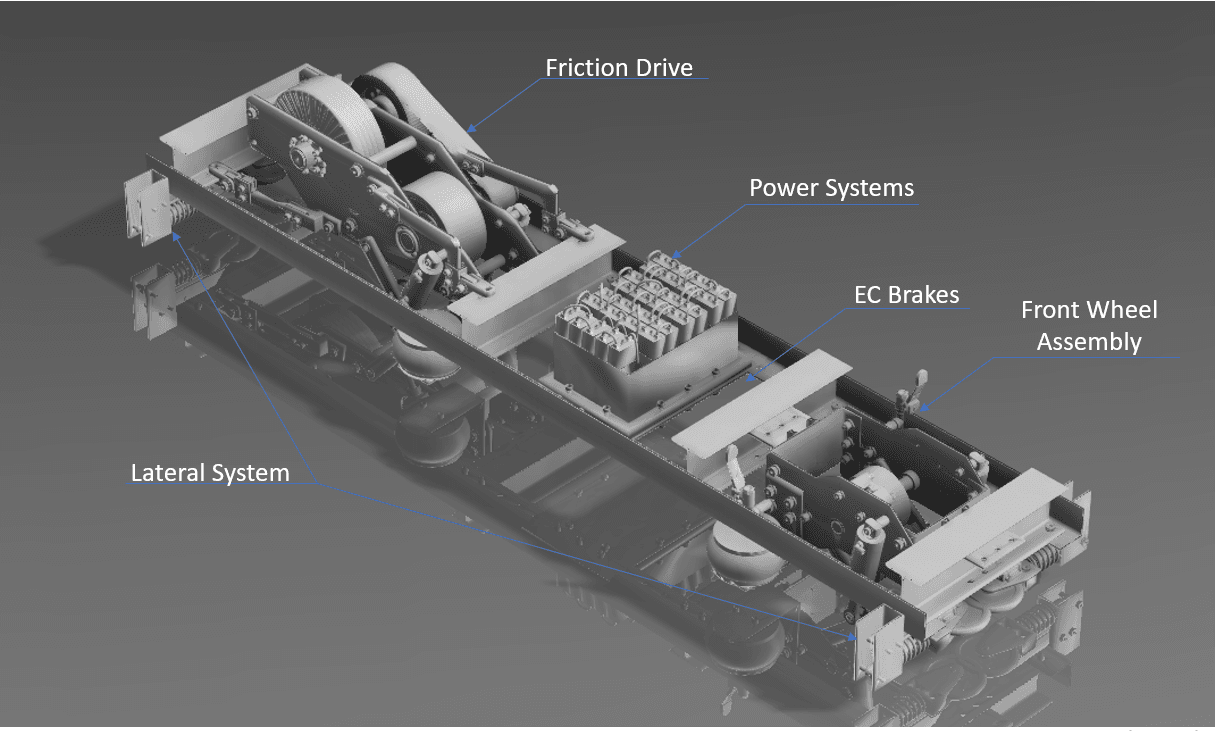
\includegraphics[width=\linewidth]{images/jimmypictwopointoh.png}
        \caption{CAD of Overall Design}
    \end{figure}

Our pod design process for Competition III began with the goal of building the fastest pod. Based purely on specific power and energy of lithium ion batteries (and perhaps supercapacitors), it is theoretically possible to achieve speeds above Mach 1 within the 1-mile Hyperloop test track. This year, our pod is designed to achieve \SI{100}{m/s}, and we are gradually working towards higher and higher speeds for future competitions.

\section{Summary of design}
Our pod consists of the following major components:
\begin{itemize}
    \item Propulsion: Friction drive (wheels)
    \item Braking: High speed eddy current braking, low speed caliper brakes
    \item Lateral stability: Freely spinning wheels
    \item Frame: Aluminum ladder frame
\end{itemize}

\subsection{Size and Mass}
The size of the pod is primarily dictated by the size of the propulsion system and the size of the I-beam.\\
  The mass of the pod depends on the individual mass of each subsystem, as seen in \reftab{table:mass}. The overall mass of the pod should be approximately 149 kilograms.

\begin{table}[H]
\centering
\begin{tabular}{@{}lr@{}}
	\toprule Subsystem & Mass of Subsystem (\si{kg}) \\ \midrule
    Friction Drive & 55.8 \\
    Frame & 19.0 \\
    Electrical & 23.5 \\
    Embedded Systems & 2 \\
    Shell & 12.0 \\
    Eddy Current Braking & 27.0 \\
    Lateral & 10.1 \\ \midrule
    \textbf{Total} & \textbf{149.4}
\end{tabular}
  \caption{Mass of Individual Subsystems}
  \label{table:mass}
\end{table}


\subsection{Energy Storage and Usage}
Energy in the pod is stored in:
\begin{itemize}
    \item Huge batteries
    \item Air tanks
    \item Lateral/EC Brakes springs
\end{itemize}
Energy is used in the pod by:
\begin{itemize}
    \item Friction drive
    \item Electronic systems (electrically isolated)
\end{itemize}


\subsection{Loading and Unloading Plan}
Due to the pod being relatively lightweight – approximately 149 kilograms, the pod can simply be moved and lifted by 10 people. This distributes the mass to \SI{15}{kg} per person. Therefore, moving to and away from the Hyperloop competition is not a large safety concern.
\section{Scalability}
Our pod design seeks to be the simplest possible design for a Hyperloop. However, it is difficult to scale to high-subsonic speeds for several reasons.
In order to fully do so, the team will eventually need to gain experience with high power systems, high speed stability, and braking systems on a larger scale. The core concept of friction drive, that is, high-speed wheeled propulsion, is not very scalable. This is because the wheel rpm increases linearly with speed and centripetal force required increases with the square of the rpm. This means that at high speeds, the wheel faces very high stresses. This problem especially affects wheels of small radius, which have a higher rpm than wheels of a larger radius. However, the friction drive can be used for low speed control where other propulsion methods, such as a linear induction motor, are less efficient, or do not work outright. Additionally, there are sections of the friction drive that are still scalable to larger pod masses and velocities. The most prominent example is the suspension system, made up of a Watts linkage and airbag suspension units. Airbag suspensions are used in industrial applications where they bear high loads, such as in trains and semi trucks. The Watts linkage is a linkage used to allow vertical movement while restricting all other directions, and is used in older train suspension designs and off road trucks. The linkage is quite simple in design, and easy to implement in tight spaces. Since Waterloop is looking to use the friction drive as a segue into more speed-specific propulsion methods, such as a high speed LIM, its lack of scalability is not a particularly troublesome issue in our Hyperloop design.\\

\end{document}